\documentclass[a4paper,12pt,twoside]{memoir}

% Castellano
\usepackage[spanish,es-tabla]{babel}
\selectlanguage{spanish}
\usepackage[utf8]{inputenc}
\usepackage[T1]{fontenc}
\usepackage{lmodern} % Scalable font
\usepackage{microtype}
\usepackage{placeins}
\usepackage{titling}
\usepackage{float}
\usepackage{tablefootnote}
\usepackage{longtable}

\RequirePackage{booktabs}
\RequirePackage[table]{xcolor}
\RequirePackage{xtab}
\RequirePackage{multirow}

% Links
\usepackage[colorlinks]{hyperref}
\hypersetup{
	allcolors = {red}
}

% Ecuaciones
\usepackage{amsmath}

% Rutas de fichero / paquete
\newcommand{\ruta}[1]{{\sffamily #1}}

% Párrafos
\nonzeroparskip


% Imagenes
\usepackage{graphicx}
\newcommand{\imagen}[2]{
	\begin{figure}[!h]
		\centering
		\includegraphics[width=0.9\textwidth]{#1}
		\caption{#2}\label{fig:#1}
	\end{figure}
	\FloatBarrier
}

\newcommand{\imagenflotante}[2]{
	\begin{figure}%[!h]
		\centering
		\includegraphics[width=0.9\textwidth]{#1}
		\caption{#2}\label{fig:#1}
	\end{figure}
}



% El comando \figura nos permite insertar figuras comodamente, y utilizando
% siempre el mismo formato. Los parametros son:
% 1 -> Porcentaje del ancho de página que ocupará la figura (de 0 a 1)
% 2 --> Fichero de la imagen
% 3 --> Texto a pie de imagen
% 4 --> Etiqueta (label) para referencias
% 5 --> Opciones que queramos pasarle al \includegraphics
% 6 --> Opciones de posicionamiento a pasarle a \begin{figure}
\newcommand{\figuraConPosicion}[6]{%
  \setlength{\anchoFloat}{#1\textwidth}%
  \addtolength{\anchoFloat}{-4\fboxsep}%
  \setlength{\anchoFigura}{\anchoFloat}%
  \begin{figure}[#6]
    \begin{center}%
      \Ovalbox{%
        \begin{minipage}{\anchoFloat}%
          \begin{center}%
            \includegraphics[width=\anchoFigura,#5]{#2}%
            \caption{#3}%
            \label{#4}%
          \end{center}%
        \end{minipage}
      }%
    \end{center}%
  \end{figure}%
}

%
% Comando para incluir imágenes en formato apaisado (sin marco).
\newcommand{\figuraApaisadaSinMarco}[5]{%
  \begin{figure}%
    \begin{center}%
    \includegraphics[angle=90,height=#1\textheight,#5]{#2}%
    \caption{#3}%
    \label{#4}%
    \end{center}%
  \end{figure}%
}
% Para las tablas
\newcommand{\otoprule}{\midrule [\heavyrulewidth]}
%
% Nuevo comando para tablas pequeñas (menos de una página).
\newcommand{\tablaSmall}[5]{%
 \begin{table}
  \begin{center}
   \rowcolors {2}{gray!35}{}
   \begin{tabular}{#2}
    \toprule
    #4
    \otoprule
    #5
    \bottomrule
   \end{tabular}
   \caption{#1}
   \label{tabla:#3}
  \end{center}
 \end{table}
}

%
% Nuevo comando para tablas pequeñas (menos de una página).
\newcommand{\tablaSmallSinColores}[5]{%
 \begin{table}[H]
  \begin{center}
   \begin{tabular}{#2}
    \toprule
    #4
    \otoprule
    #5
    \bottomrule
   \end{tabular}
   \caption{#1}
   \label{tabla:#3}
  \end{center}
 \end{table}
}

\newcommand{\tablaApaisadaSmall}[5]{%
\begin{landscape}
  \begin{table}
   \begin{center}
    \rowcolors {2}{gray!35}{}
    \begin{tabular}{#2}
     \toprule
     #4
     \otoprule
     #5
     \bottomrule
    \end{tabular}
    \caption{#1}
    \label{tabla:#3}
   \end{center}
  \end{table}
\end{landscape}
}

%
% Nuevo comando para tablas grandes con cabecera y filas alternas coloreadas en gris.
\newcommand{\tabla}[6]{%
  \begin{center}
    \tablefirsthead{
      \toprule
      #5
      \otoprule
    }
    \tablehead{
      \multicolumn{#3}{l}{\small\sl continúa desde la página anterior}\\
      \toprule
      #5
      \otoprule
    }
    \tabletail{
      \hline
      \multicolumn{#3}{r}{\small\sl continúa en la página siguiente}\\
    }
    \tablelasttail{
      \hline
    }
    \bottomcaption{#1}
    \rowcolors {2}{gray!35}{}
    \begin{xtabular}{#2}
      #6
      \bottomrule
    \end{xtabular}
    \label{tabla:#4}
  \end{center}
}

%
% Nuevo comando para tablas grandes con cabecera.
\newcommand{\tablaSinColores}[6]{%
  \begin{center}
    \tablefirsthead{
      \toprule
      #5
      \otoprule
    }
    \tablehead{
      \multicolumn{#3}{l}{\small\sl continúa desde la página anterior}\\
      \toprule
      #5
      \otoprule
    }
    \tabletail{
      \hline
      \multicolumn{#3}{r}{\small\sl continúa en la página siguiente}\\
    }
    \tablelasttail{
      \hline
    }
    \bottomcaption{#1}
    \begin{xtabular}{#2}
      #6
      \bottomrule
    \end{xtabular}
    \label{tabla:#4}
  \end{center}
}

%
% Nuevo comando para tablas grandes sin cabecera.
\newcommand{\tablaSinCabecera}[5]{%
  \begin{center}
    \tablefirsthead{
      \toprule
    }
    \tablehead{
      \multicolumn{#3}{l}{\small\sl continúa desde la página anterior}\\
      \hline
    }
    \tabletail{
      \hline
      \multicolumn{#3}{r}{\small\sl continúa en la página siguiente}\\
    }
    \tablelasttail{
      \hline
    }
    \bottomcaption{#1}
  \begin{xtabular}{#2}
    #5
   \bottomrule
  \end{xtabular}
  \label{tabla:#4}
  \end{center}
}



\definecolor{cgoLight}{HTML}{EEEEEE}
\definecolor{cgoExtralight}{HTML}{FFFFFF}

%
% Nuevo comando para tablas grandes sin cabecera.
\newcommand{\tablaSinCabeceraConBandas}[5]{%
  \begin{center}
    \tablefirsthead{
      \toprule
    }
    \tablehead{
      \multicolumn{#3}{l}{\small\sl continúa desde la página anterior}\\
      \hline
    }
    \tabletail{
      \hline
      \multicolumn{#3}{r}{\small\sl continúa en la página siguiente}\\
    }
    \tablelasttail{
      \hline
    }
    \bottomcaption{#1}
    \rowcolors[]{1}{cgoExtralight}{cgoLight}

  \begin{xtabular}{#2}
    #5
   \bottomrule
  \end{xtabular}
  \label{tabla:#4}
  \end{center}
}


\graphicspath{ {./img/} }

% Capítulos
\chapterstyle{bianchi}
\newcommand{\capitulo}[2]{
	\setcounter{chapter}{#1}
	\setcounter{section}{0}
	\chapter*{#2}
	\addcontentsline{toc}{chapter}{#1. #2}
	\markboth{#2}{#2}
}

% Apéndices
\renewcommand{\appendixname}{Apéndice}
\renewcommand*\cftappendixname{\appendixname}

\newcommand{\apendice}[1]{
	%\renewcommand{\thechapter}{A}
	\chapter{#1}
}

\renewcommand*\cftappendixname{\appendixname\ }

% Formato de portada
\makeatletter
\usepackage{xcolor}
\newcommand{\tutor}[1]{\def\@tutor{#1}}
\newcommand{\course}[1]{\def\@course{#1}}
\definecolor{cpardoBox}{HTML}{E6E6FF}
\def\maketitle{
  \null
  \thispagestyle{empty}
  % Cabecera ----------------
\begin{center}%
	{\noindent\Huge Universidades de Burgos, León y Valladolid}\vspace{.5cm}%
	
	{\noindent\Large Máster universitario}\vspace{.5cm}%
	
	{\noindent\Huge \textbf{Inteligencia de Negocio y Big~Data en Entornos Seguros}}\vspace{.5cm}%
\end{center}%

\begin{center}%
	
\includegraphics[height=3cm]{img/escudoUBU} \hspace{1cm}
	
\includegraphics[height=3cm]{img/escudoUVA} \hspace{1cm}
	
\includegraphics[height=3cm]{img/escudoULE} \vspace{1cm}%
\end{center}%

  \vfill
  % Título proyecto y escudo informática ----------------
  \colorbox{cpardoBox}{%
    \begin{minipage}{.9\textwidth}
      \vspace{.5cm}\Large
      \begin{center}
      \textbf{\LARGE\@title{}}
      \end{center}
      \vspace{.2cm}
    \end{minipage}

  }%
  \hfill
  \vfill
  % Datos de alumno, curso y tutores ------------------
  \begin{center}%
  {%
    \noindent\LARGE
    Presentado por \@author{}\\ 
    en Universidad de Burgos --- \@date{}\\
    Tutor: \@tutor{}\\
  }%
  \end{center}%
  \null
  \cleardoublepage
  }
\makeatother

\newcommand{\nombre}{José Luis Garrido Labrador} %%% cambio de comando

% Datos de portada
\title{Arquitectura \textit{Big Data} de colas para el procesado de vídeo en tiempo real}
\author{\nombre}
\tutor{Dr. Álvar Arnaiz González y Dr. José Francisco Díez Pastor}
\date{\today}

\begin{document}

\maketitle


\newpage\null\thispagestyle{empty}\newpage


%%%%%%%%%%%%%%%%%%%%%%%%%%%%%%%%%%%%%%%%%%%%%%%%%%%%%%%%%%%%%%%%%%%%%%%%%%%%%%%%%%%%%%%%
\thispagestyle{empty}


\noindent
\begin{center}%
	{\noindent\Huge Universidades de Burgos, León y Valladolid}\vspace{.5cm}%
	
\begin{center}%
	
\includegraphics[height=3cm]{img/escudoUBU} \hspace{1cm}
	
\includegraphics[height=3cm]{img/escudoUVA} \hspace{1cm}
	
\includegraphics[height=3cm]{img/escudoULE} \vspace{1cm}%
\end{center}%

	{\noindent\Large \textbf{Máster universitario en Inteligencia de Negocio y Big~Data en Entornos Seguros}}\vspace{.5cm}%
\end{center}%



\noindent Dr. D. Álvar Arnaiz González, profesor del departamento de Ingeniería Informática.

\noindent Expone:

\noindent Que el alumno D. \nombre, con DNI 71707244Y, ha realizado el Trabajo final de Máster en Inteligencia de Negocio y Big Data en Entornos Seguros 
          titulado \thetitle. 

\noindent Y que dicho trabajo ha sido realizado por el alumno bajo la dirección del que suscribe, en virtud de lo cual se autoriza su presentación y defensa.

\begin{center} %\large
En Burgos, {\large \today}
\end{center}

\vfill\vfill\vfill

% Author and supervisor
\begin{minipage}{0.45\textwidth}
\begin{flushleft} %\large
Vº. Bº. del Tutor:\\[2cm]
Dr. D. Álvar Arnaiz González
\end{flushleft}
\end{minipage}
\hfill
\begin{minipage}{0.45\textwidth}
\begin{flushleft} %\large
Vº. Bº. del co-tutor:\\[2cm]
Dr. D. José Francisco Díez Pastor
\end{flushleft}
\end{minipage}
\hfill

\vfill

% para casos con solo un tutor comentar lo anterior
% y descomentar lo siguiente
%Vº. Bº. del Tutor:\\[2cm]
%D. nombre tutor


\newpage\null\thispagestyle{empty}\newpage




\frontmatter

% Abstract en castellano
\renewcommand*\abstractname{Resumen}
\begin{abstract}
En este primer apartado se hace una \textbf{breve} presentación del tema que se aborda en el proyecto.
\end{abstract}

\renewcommand*\abstractname{Descriptores}
\begin{abstract}
Palabras separadas por comas que identifiquen el contenido del proyecto Ej: servidor web, buscador de vuelos, android \ldots
\end{abstract}

\clearpage

% Abstract en inglés
\renewcommand*\abstractname{Abstract}
\begin{abstract}
A \textbf{brief} presentation of the topic addressed in the project.
\end{abstract}

\renewcommand*\abstractname{Keywords}
\begin{abstract}
keywords separated by commas.
\end{abstract}

\clearpage

% Indices
\tableofcontents

\clearpage

\listoffigures

\clearpage

\listoftables
\clearpage

\mainmatter

\addcontentsline{toc}{part}{Memoria}
\part*{Memoria}

\capitulo{1}{Introducción}

La creciente facilidad para el acceso a Internet de alta velocidad por parte de la población del primer mundo ha permitido que los servicios de salud puedan llegar de manera telemática a la población alejada físicamente de los centros de salud y algunas tareas, como la rehabilitación de paciente de la enfermedad de Parkinson, se puede realizar con los modernos sistemas de videoconferencia.

Esta nueva forma de conexión entre terapeutas ocupacionales y sus pacientes puede ser apoyada con técnicas de inteligencia artificial. Estas pueden apoyar al terapeuta con su tarea rehabilitadora con información en tiempo real, incluso ayudar a la rehabilitación de muchos más pacientes a la vez. Para esta tarea, es necesaria tanto una determinada infraestructura técnica capaz de soportar y gestionar correctamente la carga de datos en tiempo real, como unos determinados modelos de inteligencia artificial capaces de procesar la información haciendo con un coste mínimo en tiempo y memoria.

Este trabajo de fin de máster está integrado en el proyecto \textit{Estudio de factibilidad y coste-efectividad del uso telemedicina con un equipo multidisciplinar para prevención de caídas en la enfermedad de Parkinson} del Ministerio de ciencia, innovación y universidades. Expediente \textbf{PI19/00670}. 

El objetivo de este trabajo consiste en la creación de la arquitectura de colas para el procesado de los vídeos de los pacientes en tiempo real en un entorno \textit{Big Data}. Además del aquí presentado existe otro TFM, desarrollado por el alumno José Miguel Ramírez Sanz, cuyo objetivo es la creación del algoritmo para el procesamiento del vídeo. Ambos trabajos dan el soporte informático al proyecto indicado.

\section{Material adjunto}

Junto a esta memoria se incluyen

\begin{itemize}
	\item \textbf{Anexos} donde se incluyen:
	\begin{itemize}
		\item Plan de proyecto
		\item Diseño del sistema
		\item Manual para el programador
		\item Manual para el usuario realizado junto a José Miguel Ramírez Sanz
	\end{itemize}
	\item \textit{Scripts} para el despliegue del sistema de colas para una instalación sobre máquinas \textit{Docker}.
\end{itemize}

Además se puede acceder a través de Internet al \href{https://github.com/jlgarridol/TFM-IF-FIS}{repositorio GitHub del proyecto}.
\capitulo{2}{Objetivos del proyecto}
Los objetivos del proyecto se han dividido en tres apartados siendo estos los objetivos generales, los técnicos y los personales.

\section{Objetivos generales}

\begin{itemize}
	\item Exploración de las diferentes herramientas para el procesado de vídeo en tiempo real a través de las fases de emisión, recogida, encolado, ingestión, procesado, enriquecimiento y almacenamiento.
	\item Estudio del estado del arte en análisis de imagen para problemas de salud ante distintos escenarios tanto en aspectos físicos (iluminación, enfoque...) como en aspectos lógicos (resolución, tasa de refresco...).
	\item Implementación del software necesario para la recogida de vídeo en tiempo real sobre sistemas de videoconferencia.
\end{itemize}

\section{Objetivos técnicos}

\begin{itemize}
	\item Crear una infraestructura software basada en contenedores \textit{Docker} para ser independientes del software anfitrión.
	\item Desplegar un \textit{pipeline} sobre herramientas de la suite de \textit{Apache} para el \textit{Big Data} que satisfagan el flujo ETL propuesto (TODO Cita al flujo).
	\item Desarrollar algoritmo sobre \textit{Spark Stream} que procese los vídeos generando los datos necesarios para los estudios posteriores. 
\end{itemize}


\section{Objetivos personales}

\begin{itemize}
	\item Contribuir a la mejora de la calidad de vida a través de facilitar soportes para la rehabilitación de pacientes de Parkinson.
	\item Conocer más profundamente las herramientas de la suite de \textit{Apache} y como estas se pueden combinar para facilitar tareas de \textit{Big Data}.
	\item Completas mi formación durante el máster a través de la creación de una solución que utiliza gran parte de los conocimientos adquiridos durante el mismo.
\end{itemize}


\capitulo{3}{Conceptos teóricos}


En este capítulo se explicarán los conceptos teóricos subyacentes a todos los apartados del proyecto. Se afrontará en tres bloques: primero respecto a la teoría sobre la computación distribuida (\autoref{sec:tecdis}), otro sobre los flujos de datos (\autoref{sec:tecstream}) y,  por último, sobre la manipulación de imágenes (\autoref{sec:teccv}).

\section{Computación distribuida}\label{sec:tecdis}

Se denomina computación distribuida a las técnicas software para la gestión y el desarrollo sobre sistemas en los que sus componentes físicos y lógicos están separados y se comunican físicamente por red y lógicamente por paso de mensaje~\cite{wiki:computaciondistribuida}.

Es importante destacar que la computación distribuida no tiene una relación directa con la computación paralela~\cite{christos1994computational}, es decir, aquella que se ejecuta en diversos hilos de ejecución. 

La computación paralela no tiene por que ser distribuida ni viceversa. Sin embargo, es habitual que la computación distribuida sea paralela o el servicio se dé paralelamente a diferentes aplicaciones. Un caso típico de computación distribuida y paralela puede ser el de un servicio web. Cada conexión con el servidor es un hilo diferente de ejecución y los recursos necesarios para ofrecer el servicio (bases de datos, procesadores de información, etc.) estén distribuidos en la red.

Debido a que los sistemas que procesan \textit{Big Data} necesitan una gran cantidad de almacenamiento junto con herramientas que lo gestionen de la manera más eficiente posible, la mayoría de estos sistemas son distribuidos y paralelos.


\section{Flujos de datos}\label{sec:tecstream}

Un flujo de datos es una estructura de datos continua con elementos ilimitados que aparecen en orden secuencial y no permite acceso aleatorio a los datos. Por este motivo el conjunto de datos completo, ni siquiera una gran parte de los mismos, pueden ser incluidos en la memoria principal. Como los datos son continuos se pueden procesar individualmente, en bloques (también denominados \textit{chunks}) o por ventanas deslizantes.


Por este motivo los algoritmos que procesan flujos de datos han de tener dos características principales~\cite{bifet2018machine}:

\begin{enumerate}
	\item deben procesar cada parte del flujo que lean antes de que llegue la siguiente
	\item y deben procesar los datos usando una pequeña cantidad de memoria.
\end{enumerate}

Debido a esto, los algoritmos que se ejecutan sobre los flujos se suelen enfocar a soluciones aproximadas para minimizar el uso temporal y espacial. Además, si se aplican algoritmos cuyo comportamiento dependa de la evolución del flujo y el contenido del mismo cambia en sus características estadísticas, el programa debe poder adaptarse a estos cambios.

Para la adaptación de cambios existen dos aproximaciones principales: el uso de ventanas deslizantes, para que de este modo solo se tengan en cuenta los datos más recientes, y el uso de ventanas de decaimiento, en el que se dan más peso a los datos más recientes. 

\subsection{Aplicaciones}

Los flujos de datos aparecen en multitud de entornos, principalmente en aquellos donde el tiempo real es más importante y los datos se generan continuamente.

Ejemplos de estas aplicaciones pueden ser~\cite{rodriguez2020flujos}:
\begin{itemize}
	\item Sensores en el \textit{Internet de las cosas} (\textit{IoT}),
	\item telecomunicaciones: llamadas, ubicación de los dispositivos $\ldots$,
	\item redes sociales: interacciones de los usuarios, tendencias $\ldots$,
	\item comercio electrónico: publicidad en tiempo real, actividad del usuario, detección de fraude $\ldots$,
	\item asistencia sanitaria: telemedicina, evolución de los pacientes $\ldots$
	\item o epidemias y desastres naturales: evolución de una enfermedad, propagación vírica $\ldots$.
\end{itemize}




\section{Procesamiento de imágenes}\label{sec:teccv}

A la hora de hacer procesamiento sobre vídeo, el fundamento principal es el procesamiento de los fotogramas que lo componen. Por tanto es importante entender como funcionan a nivel lógico las imágenes digitales, cómo operar con ellas y cómo procesarlas para obtener los mejores resultados.

\subsection{Definiciones}

\textbf{Imagen de 24 bits}: codificación habitual de las imágenes a color. Cada píxel se define como la combinación de tres enteros sin signo de 8 bits. La codificación (o espacio de color) necesaria para la visualización es la combinación de las capas de color roja, verde y azul, conocida como RGB, aunque también la BGR usada por openCV. 

\textbf{HSV}~\cite{wiki:hsv}: acrónimo del inglés de matiz, saturación y valor (\autoref{fig:hsv}). Consiste en un modelo de color basado en los componentes del mismo y representa una transformación no lineal del espacio de color RGB. El matiz, también conocido como tono, es el grado del ángulo respecto a la rueda de color. Representa un color único y algunos ejemplos son el rojo (0\grado), amarillo (60\grado) o verde (120\grado). La saturación representa la pureza del color entre el gris (valor mínimo) al color puro (valor máximo). El valor representa la luminosidad del color siendo el valor mínimo el color negro y el valor máximo el color con la saturación aplicada.

\begin{figure}
	\centering
	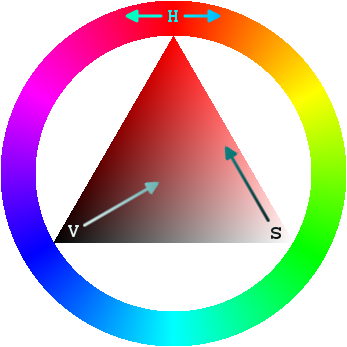
\includegraphics[width=0.5\textwidth]{Triangulo_HSV}
	\caption[Espacio de color HSV y la representación geométrica de cada componente.]{Espacio de color HSV y la representación geométrica de cada componente. Fuente: \href{https://commons.wikimedia.org/w/index.php?curid=1302915}{De Samus\_ - Trabajo propio, CC BY-SA 3.0}}
	\label{fig:hsv}
\end{figure}

\textbf{Histograma}~\cite{garrido2019opencv}: El histograma es una representación de cuántos píxeles hay para cada valor de intensidad. En él se puede ver información muy útil de la imagen como su brillo (media del histograma) o su contraste (diferencia entre el valor significativo\footnote{El valor mínimo y máximo tienden a ser siempre los mismos independientes del histograma (0 y 255 respectivamente), por eso se consideran los valores que tengan una presencia significativa, por ejemplo que sea al menos un 1\% de los vaores.} máximo y mínimo). Los procesos de ajuste del brillo y contraste se pueden observar como transformaciones del histograma.

\subsection{Ajuste automático de brillo y contraste}
Para ajustar el brillo y contraste de una imagen $\textrm{I}$ hay que seleccionar dos valores $\alpha$ y $\beta$ que se deben aplicar sobre cada píxel de la imagen tal que la ecuación sea:
\begin{equation}
\textrm{I}'(x,y) = \alpha*\textrm{I}(x,y) + \beta\label{eq:brigh}
\end{equation}
Para hacer el proceso de manera automática es necesario encontrar los valores de $\alpha$ y $\beta$ adecuados. 
El procedimiento consiste en <<estirar>> una parte del histograma de la imagen de tal manera que el contenido seleccionado del mismo abarque todo el histograma, a esto se llama \textit{corte de alas} y va controlado por un parámetro que decide la posición del corte~(\autoref{fig:alphabeta}).

Por tanto, siendo $p$ el porcentaje mínimo de la frecuencia del \textit{valor} y $\vec{h}$ el histograma de la capa \textit{valor} de HSV, el proceso es el siguiente~\cite{pklab2017bright}:

\begin{enumerate}
	\item Se calcula la frecuencia acumulada de $\vec{h}$, lo definimos como el vector~$\vec{a}$.
	\item Se actualiza el valor de $p$ con $p = p*\frac{\mathbf{max}(\vec{a})}{100*2}$
	\item Se define un valor $g_{min}$ como el valor más alto de $\vec{a}$ que sea menor que $p$, también se define un valor $g_{max}$ como el valor más pequeño de $\vec{a}$ que sea mayor que $\mathbf{max}(\vec{a})-p$
	\item Se calcula el valor de $\alpha$ como $\alpha =  \frac{255}{g_{max} - g_{min}}$\footnote{255 es el valor máximo permitido en la codificación 8 bits.}.
	\item Se calcula el valor de $\beta$ como $\beta = -g_{min} * \alpha$.
\end{enumerate}

\begin{figure}[h]
	\centering
	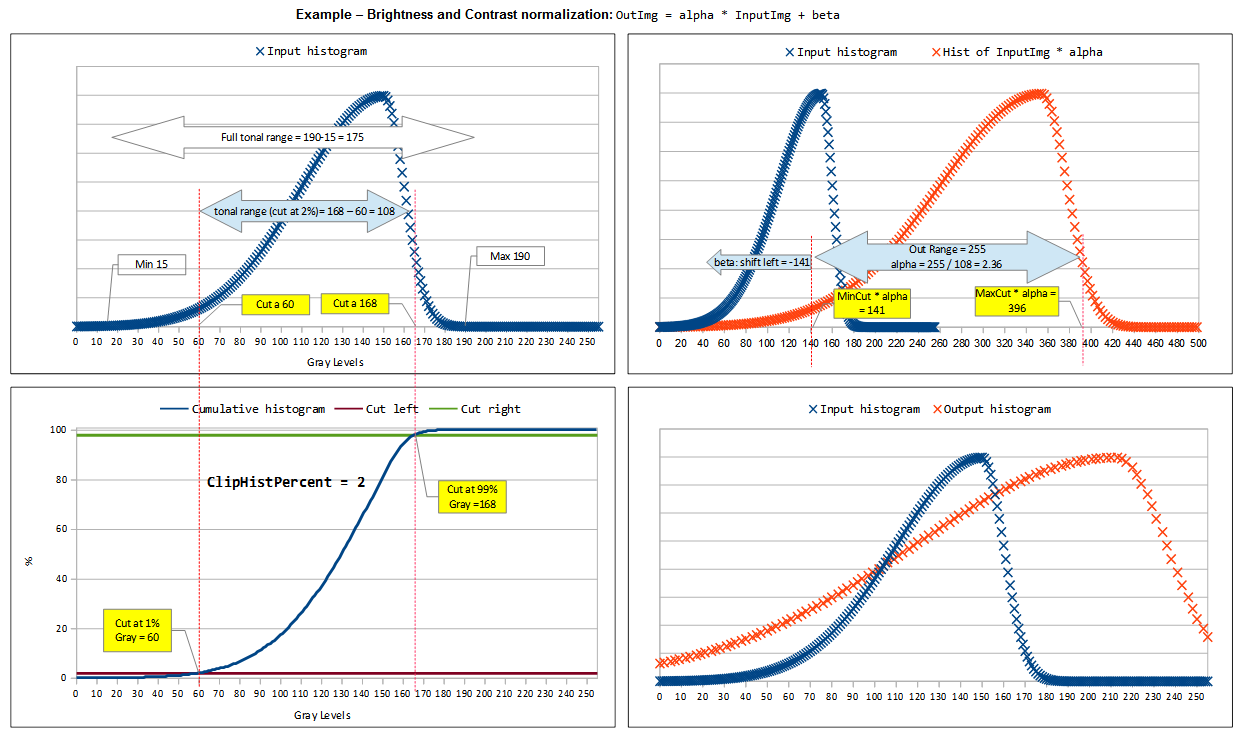
\includegraphics[width=1\textwidth]{alphabetaImageProcessing}
	\caption[Ejemplo visual del cálculo de $\alpha$ y $\beta$ para una imagen]{Ejemplo visual del cálculo de $\alpha$ y $\beta$ para una imagen. Fuente: \href{https://answers.opencv.org/question/75510/how-to-make-auto-adjustmentsbrightness-and-contrast-for-image-android-opencv-image-correction/}{De PKLab - en opencv.org}}
	\label{fig:alphabeta}
\end{figure}

En el caso de que se quisiera dejar el mismo brillo y solo cambiar el contraste, el valor de $\alpha$ a aplicar en la ecuación \eqref{eq:brigh} será 1, en caso inverso el valor de $\beta$ deberá ser 0.


\capitulo{4}{Técnicas y herramientas}

\section{Gestión de flujo}	

Uno de los puntos  esenciales de este trabajo es recoger y dirigir los \textit{streams} de vídeo que se reciben. Por tanto, escoger una correcta aplicación para la gestión de este flujo de datos es una parte muy importante dentro de las herramientas.

Dentro de la suite de \textit{Apache} existen varios componentes que se encargan de la gestión del flujos de datos. Se necesitan dos herramientas principales, una capaz de dirigir el flujo y otra para procesarlo.

\subsection{Herramientas para dirigir el flujo}
La primera herramienta necesaria debe ser capaz de dirigir flujos de datos, concretamente flujos de datos serializados para soportar datos más diversos como son las imágenes. También se necesita que sea capaz de desplegar diferentes colas para discriminar fácilmente a los distintos flujos de vídeo entrante.

En la suite de \textit{Apache} existen dos herramientas que gestionan flujos de datos, son \textit{\textbf{Apache Flume}}~\cite{noauthorapacheflume} y \textit{\textbf{Apache Kafka}}~\cite{noauthorapachenodate}.

\textit{\textbf{Apache Flume}} es herramienta de gestión de flujo diseñada para hacer una gestión distribuida de manera fiable y altamente disponible de los datos. Proporciona un servicio eficiente para la recogida, agregación y almacenamiento de los datos. Sin embargo, aunque esta herramienta pudiese suplir las necesidades de una gestión de flujo se ha descartado debido a que está optimizado para la gestión de \textit{logs}, concretamente datos codificados como cadenas, y no tiene un sistema de colas.

\textit{\textbf{Apache Kafka}} es un proyecto de intermediación de mensajes que trabaja sobre el patrón publicación-suscripción funcionando como un sistema de transacciones distribuidas. Incorpora para la implementación de este patrón un sistema de colas para la distribución de mensajes. Aporta una API para el productor, el consumidor, el flujo y el conector y la conexión se realiza a través del protocolo de la capa de transporte \textit{TCP}. Se va a utilizar esta herramienta al aportar un sistema de colas distribuidas fiable y soportar datos serializados.

\subsection{Herramientas para procesar el flujo}
En segundo lugar se necesita una herramienta capaz de procesar flujos de datos de forma escalable. La suite de \textit{Apache} tiene dos herramientas principales para el procesado de información, son \textit{\textbf{Apache Hadoop}} y \textit{\textbf{Apache Spark}}, ambas con extensiones para el procesado de flujos.

\textit{\textbf{Apache Spark Streaming}}~\cite{noauthorsparknodate} aporta una \textit{API} de consumidor nativo de \textit{Kafka}, \textit{Flume}, los sistemas de ficheros \textit{HDFS} y \textit{S3} entre otras herramientas. El funcionamiento interno consiste en crear pequeños lotes de datos para pasarlo al motor de \textit{Spark} y retornar los lotes procesados.

\textit{\textbf{Apache Hadoop Streaming}}~\cite{noauthorhadoop} tiene un funcionamiento similar a \textit{Spark Streaming} pero sin aportar de manera nativa una integración con \textit{Kafka} y \textit{Flume}.

Se ha escogido \textit{Spark Streaming} frente a \textit{Hadoop Streaming} por varios motivos:
\begin{enumerate}
	\item \textit{Spark Streaming} tiene integración con \textit{Kafka} de manera nativa.
	\item \textit{Spark Streaming} hace un uso más intensivo de la memoria RAM, por lo que es mucho más rápido si se cuenta con una gran cantidad de esta\footnote{El programa final se ha desplegado sobre una máquina con 128 GB de RAM y se ha probado en una de 32 GB de RAM con buenos resultados.}.
\end{enumerate}


\section{Infraestructura de bajo nivel}

Otro apartado importante en el despliegue de la aplicación son las herramientas y técnicas a ser usadas para la producción. Para esto se utilizan:

\begin{itemize}
	\item \textit{\textbf{GNU/Linux}}, el sistema operativo más extendido en el entorno de los servidores~\cite{noauthorred2018, zhang2000linux} además de estar disponible en los servidores prestados para la realización de este proyecto\footnote{Se utilizan el servidor \textit{Alpha} del GIR ADMIRABLE para el despliegue de la herramienta de recolección de datos (Procesador \textit{Intel Core i7}-8700, 6 núcleos, 3.2GHz. 64GB de memoria RAM. 2 GPUs GTX 1080Ti y 500GB de disco duro sólido y 6 TB de disco duro magnético) y el servidor \textit{Gamma} del mismo grupo para el despliegue de las colas y el procesado de la información (TODO Datos de gamma)}.
	\item \textit{\textbf{Docker}}, un software de gestión de contenedores estandarizados, semejante a los entornos \textit{chroot} que facilita la virtualización de software en un entorno seguro y ligero. Sobre este motor se ejecutarán las aplicaciones del entorno de \textit{Apache Spark}~\cite{juez2019docker}, \textit{Apache Kafka}~\cite{wurstmeister2019kafka} además de la aplicación desarrollada para el cumplimiento de los objetivos.
\end{itemize}

\capitulo{5}{Aspectos relevantes del desarrollo del proyecto}

Este apartado pretende recoger los aspectos más interesantes del desarrollo del proyecto, comentados por los autores del mismo.
Debe incluir desde la exposición del ciclo de vida utilizado, hasta los detalles de mayor relevancia de las fases de análisis, diseño e implementación.
Se busca que no sea una mera operación de copiar y pegar diagramas y extractos del código fuente, sino que realmente se justifiquen los caminos de solución que se han tomado, especialmente aquellos que no sean triviales.
Puede ser el lugar más adecuado para documentar los aspectos más interesantes del diseño y de la implementación, con un mayor hincapié en aspectos tales como el tipo de arquitectura elegido, los índices de las tablas de la base de datos, normalización y desnormalización, distribución en ficheros3, reglas de negocio dentro de las bases de datos (EDVHV GH GDWRV DFWLYDV), aspectos de desarrollo relacionados con el WWW...
Este apartado, debe convertirse en el resumen de la experiencia práctica del proyecto, y por sí mismo justifica que la memoria se convierta en un documento útil, fuente de referencia para los autores, los tutores y futuros alumnos.

\capitulo{6}{Trabajos relacionados}

Existe una literatura variada sobre técnicas para la rehabilitación de pacientes de la enfermedad del \textit{Parkinson} así como de aproximaciones para el análisis de vídeo en tiempo real. En este capítulo se expondrán algunos de los más relevantes.

\section{Literatura científica relacionada}

En el año 2019, Linares-del Rey \textit{et. al.}~\cite{linares2019aplicaciones} realizaron un meta-análisis sobre un total de veintiséis artículos de aplicaciones móviles para pacientes de \textit{Parkinson}. Se consideraron artículos en castellano y en inglés entre los años 2011 y 2016. Además se analizaron ciento tres aplicaciones móviles que estuviesen en los principales \textit{marketplaces}: \textit{Google Play}, \textit{App Store} y \textit{Windows Store}.

El conjunto de estudios abarcaba a un total de cuatrocientos veinte pacientes y docientos treinta y dos personas sanas, estos como grupo de control en los artículos que los incluían. 

Para valorar la calidad metodológica de estos artículos se utilizó la escala JADAD~\cite{jadad1996assessing} basada en si existe o no aleatorización de los participantes, y se describe el método, si se hace un estudio de doble ciego, y se describe el método llevado para ello, y si se describen adecuadamente las pérdidas. Se suele tomar como valor mínimo aceptable una puntación de~tres.

Entre el total de artículos revisados el único con una puntuación aceptable fue el sistema \textit{CuPid}~\cite{ginis2016feasibility} con un total de cuarenta participantes. La aplicación que presenta evaluaba la mejora de la calidad de vida del paciente según mejorasen su equilibrio, marcha y resistencia. Sin embargo, esta aplicación requería de uso de sensores externos al dispositivo móvil para poder evaluar la aplicación.

Respecto a las aplicaciones, al no tener artículos asociados (ya que de tenerlos se habrían analizado en el primer conjunto) no se podían evaluar siguiendo la misma escala. Sin embargo, algunas aplicaciones de las que se analizaron ya estaban incluidas en otras revisiones similares a las de Linares-del Rey \textit{et. al.}

La conclusión de los autores fue que debido a la baja calidad metodológica y la poca cantidad de estudios realizados, no se podía recomendar un uso generalizado de las aplicaciones, es decir, sigue haciendo falta la supervisión de terapeutas especializados que puedan dirigir y ayudar a la mejora de la calidad de vida de los pacientes.

\section{Aproximaciones en problemas similares}

El arquitecto de software Amit Baghel prensentó en 2016 una aproximación en Java para procesar vídeo utilizando \textit{Kafka} junto a \textit{Spark}~\cite{amit2017kafka}.

El objetivo de su trabajo era la creación de un detector de movimiento que combinase en una misma cola de \textit{Kafka} diferentes fuentes de vídeo y las procesase utilizando \textit{OpenCV} junto a \textit{Spark Streaming} y comparar cada \textit{frame} con el anterior y así detectar los objetos que se hubiesen movido.

\begin{figure}[h]
	\centering
	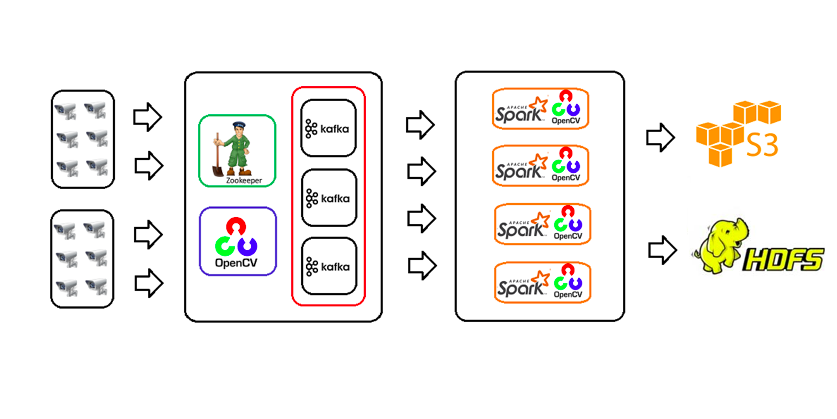
\includegraphics[width=1\textwidth]{amit}
	\caption[Diagrama de la arquitectura presentada por Amit Baghel.]{Diagrama de la arquitectura presentada por Amit Baghel. Fuente: \href{https://www.infoq.com/articles/video-stream-analytics-opencv/}{Infoq}}
\end{figure}

Debido a la similitud de la arquitectura de este trabajo con la que se deseaba contruir se utilizó como base en algunas decisiones del diseño. Concretamente se decidió mantener la configuración planteada para \textit{Kafka}: cantidad de particiones  en tres y el factor de replicación de uno.

Sin embargo, la arquitectura presentada, debido a los cambios de las versiones del los últimos años, ya no se puede desplegar en los sistemas \textit{GNU/Linux} modernos a menos que se compilen directamente las versiones que plantean.
\capitulo{7}{Conclusiones y Líneas de trabajo futuras}

Para finalizar la exposición de esta memoria se comentará en este capítulo las conclusiones del 
trabajo así como líneas futuras que se van a realizar.

\section{Conclusiones}

De este trabajo se han sacado diversas conclusiones:

\begin{itemize}
	\item Las herramientas que ofrece la \textit{suite} \textit{Apache} para la gestión y procesado de flujo son muy robustas y tiene el desempeño que se espera de ellas, especialmente referente a la flexibilidad y fiabilidad. Sin embargo, existen aún muchas limitaciones en la documentación que en la mayoría de las ocasiones es muy <<esotéricas>>, especialmente a la hora de enseñar a integrar las diversas tecnologías. De hecho, una de las mayores dificultades encontradas para el cumplimiento de los objetivos de este TFM ha sido la integración correcta de las herramientas.
	\item Los objetivos del proyecto han sido cumplidos al completo, habiendo conseguido tanto una aplicación sencilla para comunicar a pacientes y usuarios como también una arquitectura fundada sobre una tecnología robusta para facilitar el análisis en tiempo real. Se espera que esto conlleve una mejora continua de la calidad de vida de los pacientes de la enfermedad de \textit{Parkinson} al tener un acceso más fácil a los profesionales de la terapia ocupacional.
\end{itemize}

\section{Líneas futuras}

Dentro de las líneas futuras están:

\begin{itemize}
	\item Integrar el flujo con la aplicación de \textit{Jitsi} para que funcione automáticamente con los pacientes.
	\item Desplegar su uso con terapeutas y pacientes reales a una mayor escala. Actualmente se tienen tres pacientes y un terapeuta, pero el objetivo a largo plazo es que la herramienta se pueda usar por una cantidad mayor de personas.
	\item Automatizar el despliegue en clúster de servidores utilizando \textit{Kubernetes}~\cite{losautoresdekubernetes2020}, herramienta creada por \textit{Google} que permite la creación fácil de un clúster de máquinas virtuales \textit{Docker} lo que permetiría una mayor versatilidad sobre los \textit{scripts} creados en este trabajo.
	\item Explorar mejores configuraciones para \textit{Kafka} y \textit{Spark Streaming} para mejorar el desempeño del flujo.
\end{itemize}


%\renewcommand\chaptername{Anexo}
%\renewcommand\thechapter{\Roman{chapter}}
%\setcounter{chapter}{0}

% Añadir entrada en el índice: Anexos
\appendix
\addcontentsline{toc}{part}{Apéndices}
\part*{Apéndices}

\apendice{Plan de Proyecto Software}

\section{Introducción}

En este apéndice se expondrán los distintos \textit{sprints} que se han realizado y un estudio de la viabilidad del proyecto.

\section{Planificación temporal}

La planificación temporal se ha realizado adaptando la metodología \textit{Scrum}. Para poder adaptarlo a un trabajo de una sola persona para un proyecto educativo se han considerado las siguientes indicaciones:

\begin{itemize}
	\item El desarrollo se ha basado en iteraciones o \textit{sprints} de dos semana de duración aproximadamente.
	\item Cada uno de los \textit{sprints} contiene las tareas que se realizaron en el mismo. 
	\item Cada tarea tiene un coste estimado dependiendo de lo que el programador estime conveniente siguiendo los parámetros de tiempo a emplear, dificultad técnica entre otros.
	\item Una vez concluida una tarea se especifica el coste real para poder estimar de una manera más correcta tareas de \textit{sprints} siguientes.
	\item Al finalizar cada \textit{sprint} se realiza una reunión con los tutores del proyecto.
\end{itemize}

\subsection{Sprint 0}

El \textit{sprint} 0 consistió en el desarrollo de la aplicación web para la recogida de datos para el proyecto. Es el único \textit{sprint} realizado en colaboración con el alumno José Miguel Ramírez Sanz. 

\begin{table}[H]
	\begin{tabularx}{\linewidth}{X r r}
		\toprule \textbf{Tarea} & \textbf{Est.} & \textbf{Final}\\
		\otoprule
		Diseño de la interfaz web & 3 & 3 \\
		Creación de la plantilla maestra de toda la web & 3 & 2 \\
		Creación de la plantilla base para el menú del paciente & 5 & 5 \\
		Implementación del menú del terapeuta & 2 & 2 \\
		Creación de la conexión para videollamada - Terapeuta & 1 & 1 \\
		Creación de la conexión para videollamada - Paciente & 1 & 1 \\
		Implementación del sistema de inicio de sesión & 2 & 3 \\
		Creación de \textit{plugin} para la captura y emisión del vídeo del paciente & 8 & 13 \\
		Creación de la interfaz de gestión del paciente  & 2 & 2	\\	
		\bottomrule
	\end{tabularx}
	\caption{Tareas del \textit{sprint} 0}
	\label{tab:sprint0}
\end{table}

La mayor dificultad en este \textit{sprint} fue la creación del \textit{plugin} sobre \textit{Jitsi} que duplicase el flujo de vídeo y emitiese los datos del servidor al sistema de colas. Esto fue debido a la poca documentación de \textit{Jitsi} sobre la implantación de estas modificaciones. 


\subsection{Sprint 1}

El \textit{sprint} 1 consistió en la exploración de herramientas para la creación y procesado de flujos de vídeo. 

\begin{table}[H]
	\begin{tabularx}{\linewidth}{X r r}
		\toprule \textbf{Tarea} & \textbf{Est.} & \textbf{Final}\\
		\otoprule
		Búsqueda de herramientas para la creación de flujos de datos & 3 & 3 \\
		Pruebas sobre \textit{Apache Flume} & 5 & 3 \\
		Pruebas sobre \textit{Apache Kafka} & 5 & 5 \\
		Búsqueda de herramientas para el despliegue por contenedores & 3 & 3 \\
		Prueba de despliegue de \textit{Apache Kafka} para \textit{Docker} & 3 & 3 \\
		Búsqueda de herramientas para el procesado de flujos de vídeo & 3 & 3 \\
		Pruebas con \textit{Spark Streaming} con \textit{OpenCV} & 5 & 13 \\
		\bottomrule
	\end{tabularx}
	\caption{Tareas del \textit{sprint} 1}
	\label{tab:sprint1}
\end{table}

El desarrollo de este \textit{sprint} fue bastante similar a lo planificado. El caso particular estuvo en la última tarea debido a la complejidad conectar y procesar de manera efectiva \textit{Spark Streaming} con la librería de OpenCV y poder garantizar que no se perdían \textit{frames.}

\subsection{Sprint 2}

El \textit{sprint} 2 consistió en la implementación de las conexiones entre todos los elementos del flujo a nivel local. 

\begin{table}[H]
	\begin{tabularx}{\linewidth}{X r r}
		\toprule \textbf{Tarea} & \textbf{Est.} & \textbf{Final}\\
		\toprule
		Despliegue local de \textit{Apache Spark} & 2 & 2\\
		Despliegue local de \textit{Apache Kafka} & 3 & 5\\
		Simulación de servidor UDP para vídeo & 5 & 5 \\
		Ingestor a Kafka del vídeo UDP & 3 & 5\\
		Conectar \textit{Spark Streaming} con \textit{Kafka}& 3 & 13\\
		Implementar un anonimizador de rostros & 3 & 2\\
		Parametrizar todos los \textit{scripts} creados & 2 & 2	\\
		\bottomrule
	\end{tabularx}
	\caption{Tareas del \textit{sprint} 2}
	\label{tab:sprint2}
\end{table}

La razón de la gran diferencia en la quinta tarea del \textit{sprint} entre predicho e invertido fue debido a que la documentación de \textit{Kafka} no estaba bien detallada para conectar con \textit{Spark Streaming}. 

\subsection{Sprint 3}

El \textit{sprint} 3 consistió en la implementación de una infraestructura de contenedores \textit{Docker} que conectase todos los servicios para el flujo. 

\begin{table}[H]
	\begin{tabularx}{\linewidth}{X r r}
		\toprule \textbf{Tarea} & \textbf{Est.} & \textbf{Final}\\
		\otoprule
		Despliegue de \textit{Apache Spark} para el nodo \textit{master} & 2 & 2\\
		Despliegue de \textit{Apache Spark} para varios nodos \textit{worker} & 2 & 1\\
		Creación de imágenes \textit{Docker} para soportar las aplicaciones creadas & 8 & 21\\
		Despliegue de la aplicación \textit{openCV} & 3 & 3 \\
		Recogida de \textit{stream} de vídeo e ingestión en \textit{Kafka} en \textit{Docker} & 8 & 8\\
		\bottomrule
	\end{tabularx}
	\caption{Tareas del \textit{sprint} 3}
	\label{tab:sprint3}
\end{table}

Este \textit{sprint} fue más sencillo que el anterior, principalmente porque en el anterior existieron dificultades para cumplir con los plazos del mismo al complicarse la tarea de conectar dos de los componentes. Con la experiencia obtenida en ese \textit{sprint} algunas tareas se desarrollaron más fácilmente. Por otro lado el despliegue con \textit{docker} necesitó casi un \textit{sprint} aparte ya que muchas de las operaciones, a \textit{priori} simples, resultaron tener varias capas de complejidad no previstas. Esto causó el mayor desajuste entre lo previsto y lo invertido de todo el proyecto, presumiblemente por la poca experiencia previa en el uso de contenedores \textit{docker}.

\subsection{Sprint 4}

El \textit{sprint} 4 consistió en la automatización de los procesos del \textit{sprint} 3. 

\begin{table}[H]
	\begin{tabularx}{\linewidth}{X r r}
		\toprule \textbf{Tarea} & \textbf{Est.} & \textbf{Final}\\
		\otoprule
		\textit{Script} para la creación de \textit{topics} de \textit{Kafka} & 1 & 1\\
		\textit{Script} de lanzamiento de instancia del flujo & 8 & 13 \\
		\textit{Script} de inicialización de los servicios & 2 & 2\\
		\textit{Script} para la eliminiación de un \textit{topic} de \textit{Kafka} & 1 & 1\\
		\textit{Script} para el cierre ordenado de un flujo & 5 & 8\\
		\textit{Script} para el apagado completo de los servicios & 1 & 1\\
		\bottomrule
	\end{tabularx}
	\caption{Tareas del \textit{sprint} 4}
	\label{tab:sprint4}
\end{table}

La mayor dificultad de este \textit{sprint} estuvo en la creación de los \textit{scripts} que abarcasen tanto el inicio como el cierre de un flujo debido a que estaban involucrados tanto el inicio de las imágenes \textit{docker} asociadas, el control de identificadores (realizado mediante semáforos en forma de ficheros) y la ejecución ordenada. Por estos motivos las predicciones no fueron acertadas al complicarse la implementación.

\subsection{Sprint 5}

El \textit{sprint} 5 consistió en la creación de experimentos para evaluar el tiempo necesitado para el procesado del flujo además de la búsqueda de un sistema de serialización y compresión adecuado para el encolado de los fotogramas. 

\begin{table}[H]
	\begin{tabularx}{\linewidth}{X r r}
		\toprule \textbf{Tarea} & \textbf{Est.} & \textbf{Final}\\
		\toprule
		Diseño de los experimentos & 3 & 3\\
		Implementación de los experimentos del flujo & 5 & 13\\
		Implementación de los experimentos sobre las técnicas de serialización y compresión & 5 & 5\\
		Implementación de la recogida y visualización de los resultados & 3 & 3\\
		Análisis de los resultados & 3 & 3\\
		\bottomrule
	\end{tabularx}
	\caption{Tareas del \textit{sprint} 5}
	\label{tab:sprint5}
\end{table}

Hubo una gran dificultad a la hora de la implementación de los experimentos debido a que se quiso paralelizar la ejecución y acelerar así el proceso. Sin embargo, esto conllevó un estudio más en profundidad de las herramientas de \textit{Python} para ello.

\subsection{Sprint 6}

En este penúltimo \textit{sprint} se comenzó el despliegue real y la integración con el modelo predictivo de poses del alumno José Miguel Ramírez Sanz. 

\begin{table}[H]
	\begin{tabularx}{\linewidth}{X r r}
		\toprule \textbf{Tarea} & \textbf{Est.} & \textbf{Final}\\
		\toprule
		Implementación de la extensibilidad del flujo & 2 & 2\\
		Instalación local del flujo completo & 3 & 3\\
		Instalación de las librerías necesarias en el equipo \textit{Gamma} & 1 & 1\\
		Despliegue de las máquinas \textit{docker} en \textit{Gamma} & 1 & 1\\
		Pruebas sobre vídeos pregrabados & 2 & 2\\
		Adaptación de los \textit{dockers} para compatibilidad con \textit{Nvidia} & 8 & 13\\
		Diseño de experimentos sobre el flujo completo & 1 & 1\\
		Implementación de los experimentos & 8 & 5\\
		Análisis de los resultados & 2 & 2\\
		\bottomrule
	\end{tabularx}
	\caption{Tareas del \textit{sprint} 6}
	\label{tab:sprint6}
\end{table}

El \textit{sprint} se desarrolló con bastante facilidad respecto a otros debido principalmente a que gran parte del material necesario, como los \textit{scripts} de lanzamiento o experimentos similares, ya se habían creado anteriormente. El único problema estuvo relacionado con la adaptación de las imágenes \textit{Docker} a \textit{Nvida} ya que se requirieron muchos cambios inesperados para que funcionase adecuadamente.

\subsection{Sprint 7}

Este último \textit{sprint} consistió en la creación de la documentación del trabajo realizado. 

\begin{table}[H]
	\begin{tabularx}{\linewidth}{X r r}
		\toprule \textbf{Tarea} & \textbf{Est.} & \textbf{Final}\\
		\otoprule
		Maquetación de la plantilla & 1 & 1\\
		Escritura de la introducción & 2 & 2\\
		Escritura de los objetivos & 3 & 3\\
		Escritura de los conceptos teóricos & 5 & 5\\
		Escritura de los aspectos relevantes & 13 & 13\\
		Escritura de los trabajos relacionados & 3 & 3\\
		Escritura de las conclusiones y lineas futuras & 2 & 2\\
		Escritura del plan de proyecto & 2 & 2\\
		Escritura del diseño & 5 & 5\\
		Escritura del manual del programador & 3 & 3\\
		Creación de la presentación & 8 & 8\\  
		\bottomrule
	\end{tabularx}
	\caption{Tareas del \textit{sprint} 7}
	\label{tab:sprint7}
\end{table}


\section{Estudio de viabilidad}


\subsection{Viabilidad económica}

Debido a que este TFM está dentro de un proyecto donde también se encuentra el TFM de José Miguel Ramírez Sanz, se ha realizado el estudio de viabilidad económica de manera conjunta


En la \autoref{tab:costes_personal} se encuentran los costes total en salarios en jornada completa durante seis meses para dos empleados.

\begin{table}[H]\centering
	\begin{tabular}[]{@{}l r@{}}
		\toprule
		\textbf{Concepto} & \textbf{Coste (\euro{})} \\
		\midrule
		Salario mensual bruto~\cite{salariales} & 2\,047,78 \\
		Seguridad Social (30,04\%) & 615,15 \\
		Retención IRPF (2\%) & 28,65 \\
		Salario mensual neto & 1\,403,97 \\\hubu
		\textbf{Total 6 meses y dos empleados} &  24\,573,36 \\
		\bottomrule
	\end{tabular}
	\caption{Costes de personal.}
	\label{tab:costes_personal}
\end{table}

La \autoref{tab:costes_hardware} están las inversiones y amortizaciones  en materia de \textit{hardware}, tanto los \textit{MainFrames} para el despliegue y el cálculo como los equipos de desarrollo.


\begin{table}[H]
	\centering
	\begin{tabular}[]{@{}l r r@{}}
		\toprule
		\textbf{Concepto} & \textbf{Coste (\euro{})} & \textbf{Coste amortizado (\euro{})} \\
		\otoprule
		Ordenador de desarrollo (x2) & 950 &  59,37\\
		Dispositivos pacientes (x9) & 100 & 6,25\\
		\textit{Webcam} pacientes (x9) & 150 &9,38\\
		\textit{MainFrame Gamma}  & 3\,000 & 187,5 \\ 
		\textit{Gamma} GPU (x3) & 1\,500 &  93,75\\
		\textit{MainFrame Alpha}  & 2\,000 & 125 \\\hubu
		\textbf{Total} & 13\,650 & 853,16\\
		\bottomrule
	\end{tabular}
	\caption{Costes de \textit{hardware}.}
	\label{tab:costes_hardware}
\end{table}

Por último en la \autoref{tab:costes_servicios} se encuentran los dos servicios contratados para dar acceso a la aplicación a los pacientes.

\begin{table}[H]
	\centering
	\begin{tabular}[]{@{}l r@{}}
		\toprule
		\textbf{Servicio} & \textbf{Coste (\euro{})}\\
		\otoprule
 		Suscripción \textit{Ngrok}  & 7,33 \\
		Lineas \textit{Vodafone} (x4) & 30 \\\hubu
		\textbf{Total (por 6 meses)} & $763.68$\\
		\bottomrule
	\end{tabular}
	\caption{Costes de servicios.}
	\label{tab:costes_servicios}
\end{table}

Los costes totales se pueden observar en la \autoref{tab:costes_totales}.

\begin{table}[H]
	\centering
	\begin{tabular}[]{@{}l r@{}}
		\toprule
		\textbf{Servicio} & \textbf{Coste (\euro{})}\\
		\otoprule
		Costes de personal  & 24\,573,36 \\
		Costes de \textit{hardware} & 13\,650 \\
		Costes de servicios & $763.68$ \\\hubu
		\textbf{Total} & 38\,987,04\\
		\bottomrule
	\end{tabular}
	\caption{Costes totales.}
	\label{tab:costes_totales}
\end{table}


\subsection{Viabilidad legal}

Este proyecto se ha realizado con la ayuda de software de terceros con licencias propias que influyen sobre la viabilidad legal del proyecto.

Dentro de las licencias de las herramientas utilizadas están:
\begin{itemize}
		\item \textbf{MIT}: Esta licencia permite el uso comercial del producto, la modificación del mismo, la libre distribución y el uso privado. No tiene garantías ni responsabilidad. La única condición es hacer referencia a ella. Como no obliga a mantener la licencia ni afecta a la distribución del software que use la licencia final del producto, esta puede ser cualquiera.
		
		\item \textbf{GPLv3}: Licencia que permite uso comercial, distribución, modificación uso privado y creación de patentes. Obliga a licenciar
cualquier modificación del código o códigos que usen herramientas con esta licencia usar \textbf{GLPv3} u otras versiones.
		
		\item \textbf{Apache 2.0}: Licencia de las herramientas de Apache, tiene las mismas propiedades que la licencia GPLv3 con excepción de que no obliga a que las nuevas implementaciones con dependencias en Apache 2.0 sean licenciadas como código libre.

		\item \textbf{BSD}: Tiene características semejantes a MIT en el contexto en el que la usamos.
		
		\item \textbf{BSD 3-Clause}: Tiene características semejantes a MIT en el contexto en el que la usamos.
\end{itemize}

La licencia más restrictiva del proyecto, la \textit{GPLv3}, está asociada a las plantillas de imágenes \textit{docker} de Mario Juez Gil~\cite{juez2019docker}. Como el resto de licencias son compatibles con la \textit{GPLv3} se utiliza dicha licencia para todo el proyecto.

\subsubsection{\textit{Copyright} de terceros}

\textbf{Apache 2.0}:
\begin{itemize}
	\item \textit{Apache Kafka} - \textit{Apache Foundation}
	\item \textit{Apache Zookeeper} - \textit{Apache Foundation}
	\item \textit{Apache Spark} - \textit{Apache Foundation}
	\item \textit{Docker CP} - \textit{Confluentic}
	\item \textit{Jitsi Meet} - \textit{Jitsi}
\end{itemize}

\textbf{GPLv3}:
\begin{itemize}
	\item \textit{Clúster Spark Docker} - Mario Juez Gil
\end{itemize}

\textbf{BSD} todas sus variantes:
\begin{itemize}
	\item \textit{Caffe} - \textit{BVLC}
	\item \textit{Flask} - \textit{Pallets}
	\item \textit{Jinja} - \textit{Pallets}
	\item \textit{OpenCV} - \textit{Intel Corporation}, \textit{Xperience AI}
	\item \textit{Seaborn} - Michael Waskom
\end{itemize}

\textbf{MIT}
\begin{itemize}
	\item \textit{Bootstrap 4} - \textit{Twitter}
	\item \textit{jQuery} - \textit{JS Foundation}
\end{itemize}


\apendice{Especificación de Requisitos}

Este apartado no se como afrontarlo realmente porque los objetivos generales creo que están descritos en los objetivos del proyecto y el catálogo de requisitos y su especificación está más orientado a casos de uso.
\section{Introducción}

\section{Objetivos generales}

\section{Catalogo de requisitos}

\section{Especificación de requisitos}



\apendice{Especificación de diseño}

\section{Introducción}

El sistema completo funciona con la unión de dos subsistemas. El subsistema web que lo forman el servidor que identifica al usuario y la plataforma \textit{Jitsi} para realizar la videollamada y el subsistema de colas, que da nombre a este trabajo, que encola los \textit{frames} del vídeo y los procesa. 

En este apartado se explica como se ha diseñado el sistema completo, la comunicación entre todas sus partes, el flujo del trabajo y la composición de cada elemento.

\section{Diseño procedimental}

El procedimiento para el procesado de los vídeos (\autoref{fig:secuencias}) para cada paciente que entre en una videollamada (independientemente de que esté o no el terapeuta) se inicializa un nuevo \texttt{Ingestor} que encolará los frames que reciba. A su vez este \texttt{Ingestor} creará un procesador que consumirá los \textit{frames} y los procesará. Estos dos elementos permanecerán hasta que sean cerrados por la finalización de la conexión. Por tanto, por cada paciente conectado se procesará tan pronto como sea posible la secuencia de \textit{frames} del mismo.

\begin{figure}
	\centering
	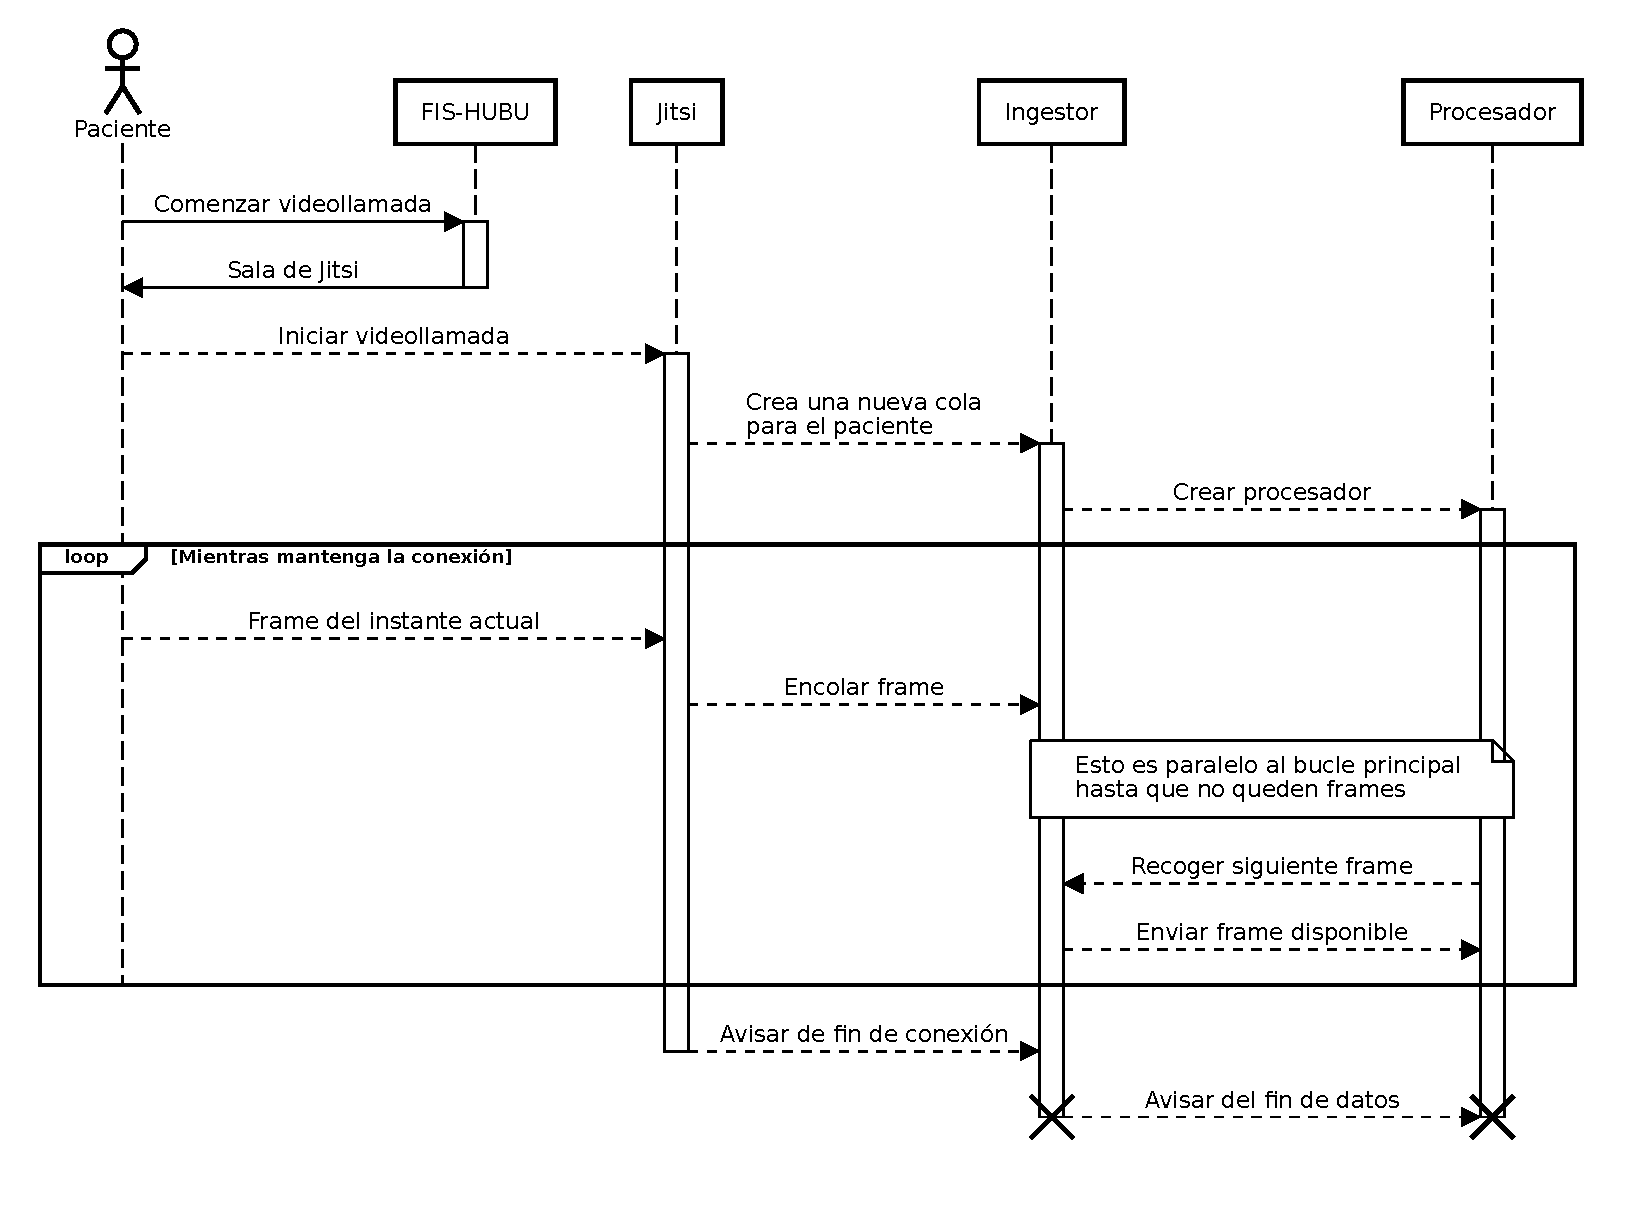
\includegraphics[width=\textwidth]{Secuencias}
	\caption[Diagrama de secuencia para el proceso general de la aplicación.]{Diagrama de secuencias para el proceso general de la aplicación. Conexión del paciente y procesado del vídeo de entrada.}
	\label{fig:secuencias}
\end{figure}



\section{Diseño arquitectónico}

La parte más esencial de este trabajo es la creación del \textit{pipeline} que procesa en tiempo real los \textit{frames} de la comunicación del paciente. Todo ello se ha desarrollado, utilizando las herramientas de la suite de \textit{Apache}, \textit{Apache Kafka} para el \textit{ingestor}, \textit{Apache Spark Streaming} para el \textit{procesador}. En la \autoref{fig:flujoetlreal} se puede observar el funcionamiento completo del flujo y las partes que lo componen.

Para que esta arquitectura sea ajena al entorno se encapsulan sobre máquinas virtuales \textit{Docker} de tal forma que se pueda desplegar en cualquier sitio. Concretamente habría cuatro tipos de imágenes \textit{Docker}. La primera se encarga de la serialización de los frames y lanzan el \textit{script} de \textit{Python} de encolado, esta máquina se crea y destruye a voluntad de las conexiones de los pacientes. La segunda y tercera imagen es el servicio de \textit{Zookeeper} y de \textit{Kafka}. Estas imágenes no se duplican en caso de cambios en las conexiones, unicamente se crean o borran colas. Por último, la cuarta imagen es la transformación del flujo. Se crean o se destruyen según las conexiones de los pacientes y se parametrizan para que consuman un flujo concreto y hagan un procesamiento concreto de tal forma que diferentes pacientes se podrían configurar para tener diferentes procesados permitiendo una mayor flexibilidad en el procesamiento.

\begin{figure}[H]
	\centering
	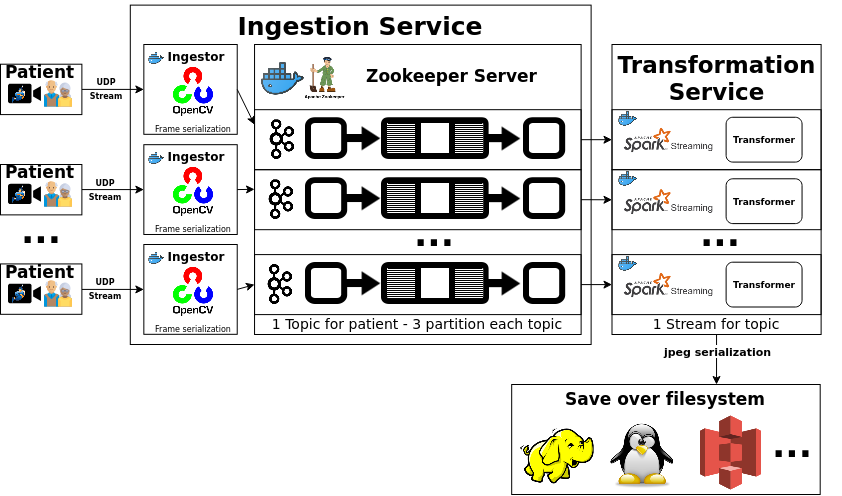
\includegraphics[width=\textwidth]{Flujo-FIS-HUBU}
	\caption[Implementación del flujo ETL para el procesado de imágenes en tiempo real.]{Implementación del flujo ETL para el procesado de imágenes en tiempo real. Por cada paciente conectado se asocia a un \textit{ingestor} que serializa la imagen y la encola en un flujo de \textit{Apache Kafka} dividido en tres particiones. Cada cola es procesada por un servidor de \textit{Apache Zookeeper}. El flujo es consumido por un procesador de \textit{Apache Spark Streaming}. El procesado puede ser cualquier operación con imágenes. Por último se almacena en el sistema de ficheros los resultados del flujo.}
	\label{fig:flujoetlreal}
\end{figure}




\apendice{Documentación técnica de programación}

\section{Introducción}

\section{Estructura de directorios}

\section{Manual del programador}

\section{Compilación, instalación y ejecución del proyecto}

\section{Pruebas del sistema}

\apendice{Documentación de usuario}

Añadir apéndice con el manual de Hutia


\bibliographystyle{plain}
\bibliography{bibliografia}

\end{document}
